\section{Lựa chọn công nghệ và lập luận}
Bảng~\ref{tab:technology} tổng hợp công nghệ, lý do lựa chọn và các hạn chế kỹ thuật cần quản lý khi phát triển hệ thống.
{\tabletext\renewcommand{\arraystretch}{1.04}\begin{longtable}{>{\raggedright\arraybackslash}p{\dimexpr0.3\textwidth-2\tabcolsep\relax}>{\raggedright\arraybackslash}p{\dimexpr0.37\textwidth-2\tabcolsep\relax}>{\raggedright\arraybackslash}p{\dimexpr0.33\textwidth-2\tabcolsep\relax}}
\caption{Công nghệ, lý do lựa chọn và hạn chế kỹ thuật}\label{tab:technology}\\
\toprule \textbf{Thành phần / phiên bản} & \textbf{Lý do lựa chọn} & \textbf{Hạn chế kỹ thuật}\\\midrule
\endfirsthead
\multicolumn{3}{l}{\small Công nghệ, lý do lựa chọn và hạn chế kỹ thuật (tiếp)}\\
\toprule \textbf{Thành phần / phiên bản} & \textbf{Lý do lựa chọn} & \textbf{Hạn chế kỹ thuật}\\\midrule
\endhead
\bottomrule\endlastfoot
React Native 0.86.2; React 19.2.3 \cite{reactnative} & Giao diện component, tái sử dụng logic TypeScript và tích hợp Android native. & Tập trung vào Android; mở rộng nền tảng cần cấu hình native tương ứng.\\\addlinespace[1.5pt]
TypeScript 5.9.3; Community CLI 20.1.0 & Kiểm kiểu model/props; kiểm soát dự án native và bridge MQTT/thông báo. & Cần quản lý Android SDK/JDK, phụ thuộc native và cấu hình build.\\\addlinespace[1.5pt]
useState/useEffect; điều hướng bằng state & Ghép các màn hình theo vai trò, truyền dữ liệu và callback trực tiếp. & Điều hướng bằng state yêu cầu xử lý BackHandler và cleanup chủ động.\\\addlinespace[1.5pt]
Async Storage 3.1.1; fetch/Promise \cite{asyncstorage} & Kho JSON local gọn và REST client thống nhất. & Hai kho local/REST độc lập; đồng bộ ngoại tuyến cần cơ chế hòa giải và bảo vệ dữ liệu.\\\addlinespace[1.5pt]
Java 17; Spring Boot 3.4.4; JPA/H2 & REST, phân quyền, giao dịch và khóa dữ liệu; H2 thuận tiện phát triển/test. & BookingService tập trung nhiều nghiệp vụ; cần phân tách khi quy mô xử lý tăng.\\\addlinespace[1.5pt]
Kotlin 2.1.20; MQTT/oneM2M & Native Android gửi lệnh khóa, nhận sự kiện và tích hợp thông báo nền tảng. & Kết nối MQTT gắn với phiên ứng dụng và cần mạng để trao đổi lệnh/sự kiện khóa.\\\addlinespace[1.5pt]
Jest 29; react-test-renderer 19.2.3 \cite{jest} & Kiểm hàm, component và hợp đồng tích hợp bằng mocks có kiểm soát. & Mock giúp kiểm tra logic có kiểm soát; thử trên thiết bị bổ sung kiểm tra tích hợp.\\\addlinespace[1.5pt]
\end{longtable}}

\subsection{React Native, TypeScript và trạng thái giao diện}
Phiên đăng nhập được quản lý ở thành phần gốc; callback xác thực cập nhật trạng thái để chuyển từ biểu mẫu sang màn hình chức năng theo vai trò. Mỗi màn giữ input/loading/error; TypeScript kiểm kiểu model, props và hợp đồng với repository \cite{react,typescript}. Community CLI cho phép tích hợp MQTT/thông báo native Android. Điều hướng và trạng thái nghiệp vụ dùng state, props và service; BackHandler, tham số, làm mới và cleanup do app xử lý trực tiếp. Khi số màn tăng, cách này cần được đánh giá lại.

\subsection{Java, Spring Boot và ánh xạ dữ liệu}
Java 17 dùng record cho request/response; Spring truyền dependency qua constructor. Controller nhận HTTP và gọi service; \code{SessionAuthFilter} kế thừa \code{OncePerRequestFilter}; \code{ApiExceptionHandler} ánh xạ ngoại lệ sang HTTP \cite{spring}. JPA/Hibernate quản lý entity/giao dịch, converter triển khai \code{AttributeConverter} cho dữ liệu JSON lồng. Entity lưu trạng thái nghiệp vụ có thể cập nhật, còn record biểu diễn dữ liệu trao đổi bất biến. H2 mặc định lưu tệp, test dùng RAM; đổi hệ quản trị vẫn cần kiểm lược đồ, truy vấn và khóa \cite{h2}.

\subsection{MQTT, oneM2M và định dạng mã khóa}
App gửi bản tin qua module Kotlin tới broker OneIoT, theo chủ đề và cấu trúc oneM2M \cite{mqtt,onem2m}. Native dùng AES/CTR/NoPadding để đóng gói mật khẩu theo định dạng thiết bị; source dẫn xuất khóa bằng SHA-256 và giá trị khởi tạo từ thời gian/số hiệu mật khẩu. Cách đóng gói này đáp ứng định dạng của thiết bị. PIN trong dữ liệu nghiệp vụ và cấu hình xác minh chứng thư TLS native là các điểm cần gia cố về bảo mật khi mở rộng vận hành.

MQTT PUBACK xác nhận broker nhận lệnh publish. App ghi trạng thái tạo/lưu/gửi mã và xử lý sự kiện khóa qua các bước riêng; chạy thử thực tế đã xác nhận luồng kết nối ứng dụng với SmartLock. Chi tiết được phân tích ở mục~\ref{sec:pin-solution}.

\FloatBarrier
\section{Kiến trúc và luồng dữ liệu}
\subsection{Ranh giới thành phần và hai nguồn dữ liệu}
Hình~\ref{fig:containers} thể hiện các thành phần chạy độc lập. Ứng dụng Android gồm giao diện React Native và native bridge; backend cung cấp REST và lưu H2; OneIoT là kết nối riêng cho khóa. App giữ phiên ở cấp gốc, còn repository chọn local hoặc REST bằng cấu hình runtimeFlags.
\begin{figure}[H]\centering
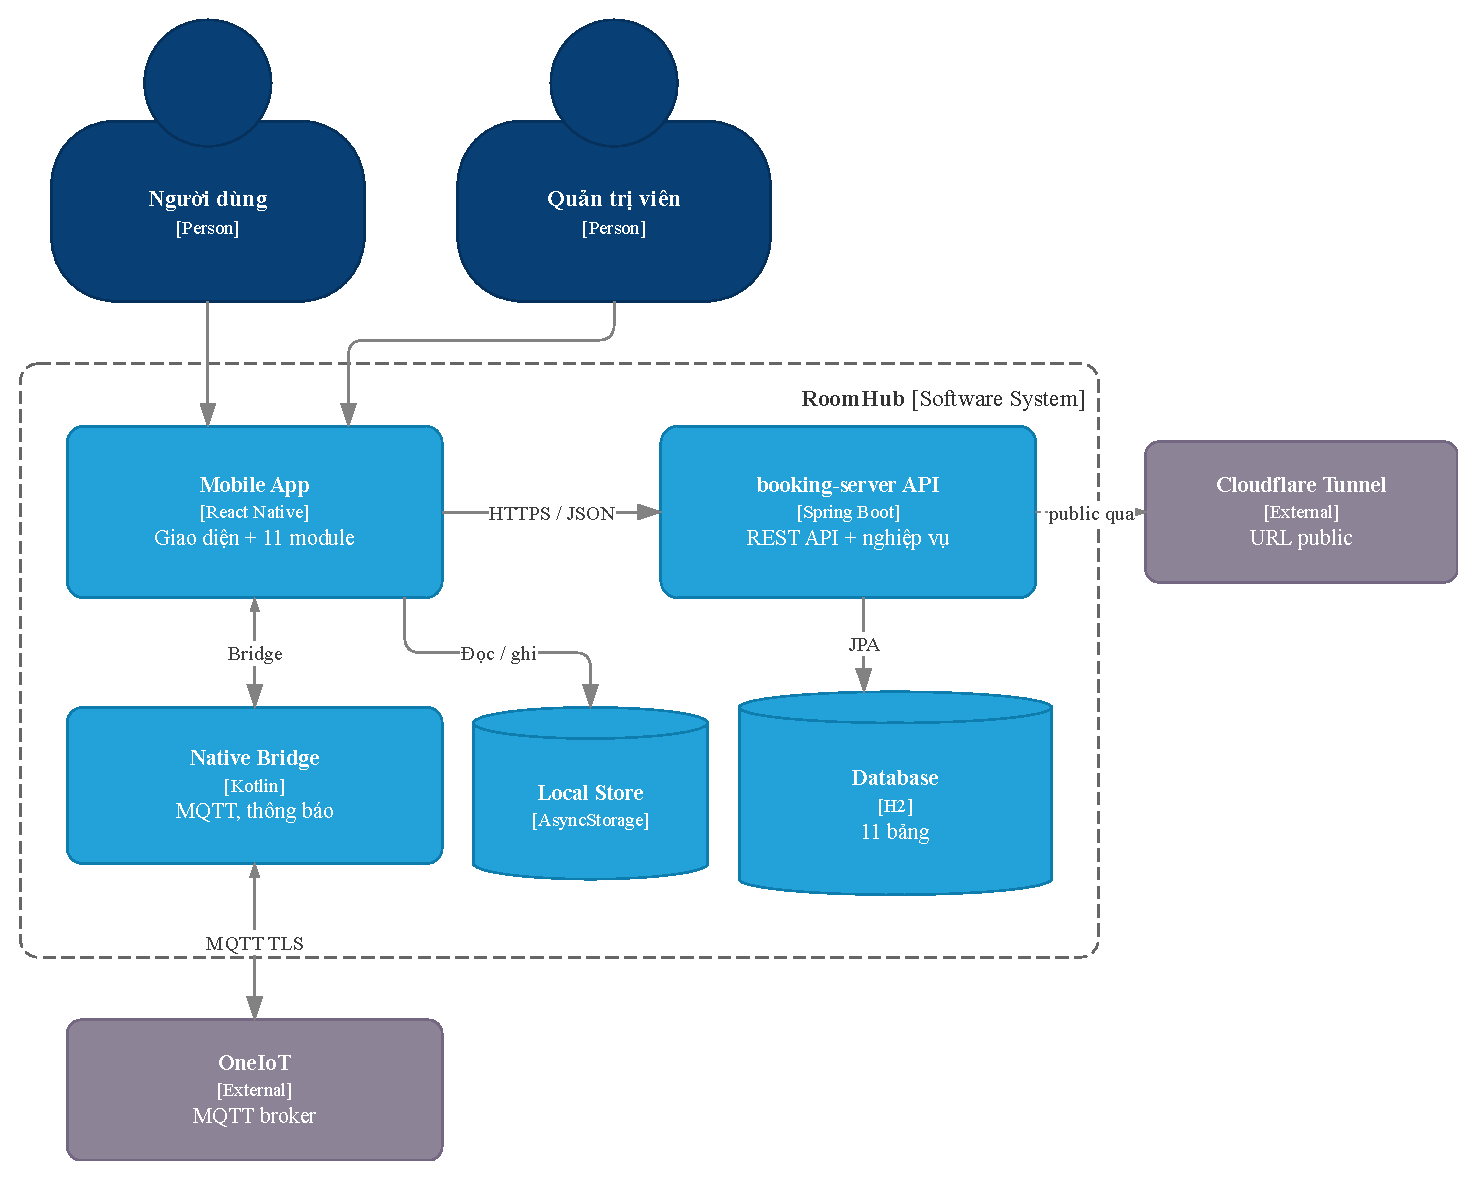
\includegraphics[width=\textwidth,height=.76\textheight,keepaspectratio]{Hinhve/design/10_c4_l2_container.pdf}
\caption{Các thành phần chạy: app Android, REST backend và OneIoT}\label{fig:containers}
\end{figure}

Luồng local là UI → repository → readJson/writeJson → Async Storage. Luồng remote là UI → apiRequest → SessionAuthFilter → controller theo nghiệp vụ → BookingService → JPA/H2. Luồng khóa là service TypeScript → module Kotlin → OneIoT theo MQTT/oneM2M. Công tắc REST không bật hoặc tắt kết nối MQTT.

Nguồn local và nguồn REST dùng cùng giao diện nghiệp vụ ở màn hình nhưng là hai kho độc lập. Chế độ REST không tự lấy backlog local, không tự hòa giải dữ liệu nhiều máy và không tự chuyển về local khi mạng lỗi. Cấu hình bản build quyết định nguồn dữ liệu sử dụng.

\subsection{Module ứng dụng và trách nhiệm lớp phía server}
Hình~\ref{fig:app-components} bổ sung cách các module cộng tác; Hình~\ref{fig:server-components} cho biết ranh giới HTTP, xác thực, nghiệp vụ và dữ liệu ở server. Hai góc nhìn làm rõ phụ thuộc giữa các module trong app và đường xử lý yêu cầu phía Java.
\begin{figure}[H]\centering
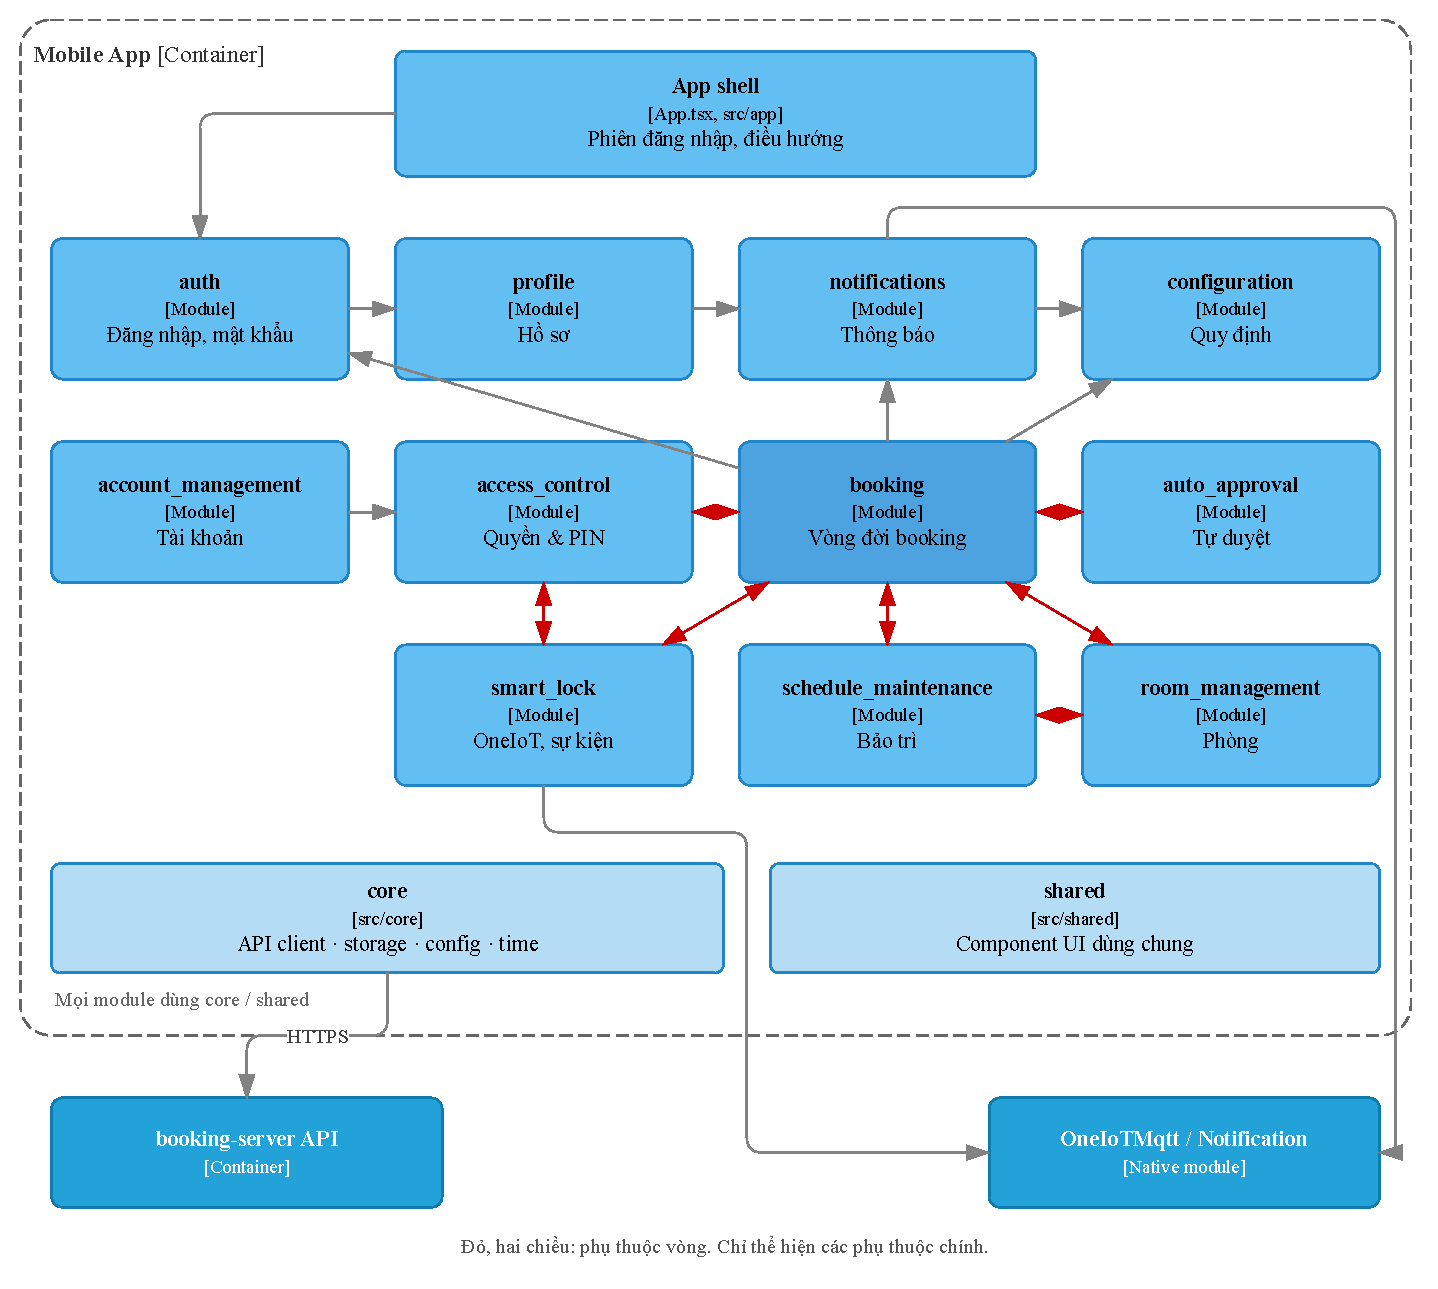
\includegraphics[width=\textwidth,height=.76\textheight,keepaspectratio]{Hinhve/design/11a_c4_l3_component_app.pdf}
\caption{Trách nhiệm và các phụ thuộc chính giữa module React Native}\label{fig:app-components}
\end{figure}
\begin{figure}[H]\centering
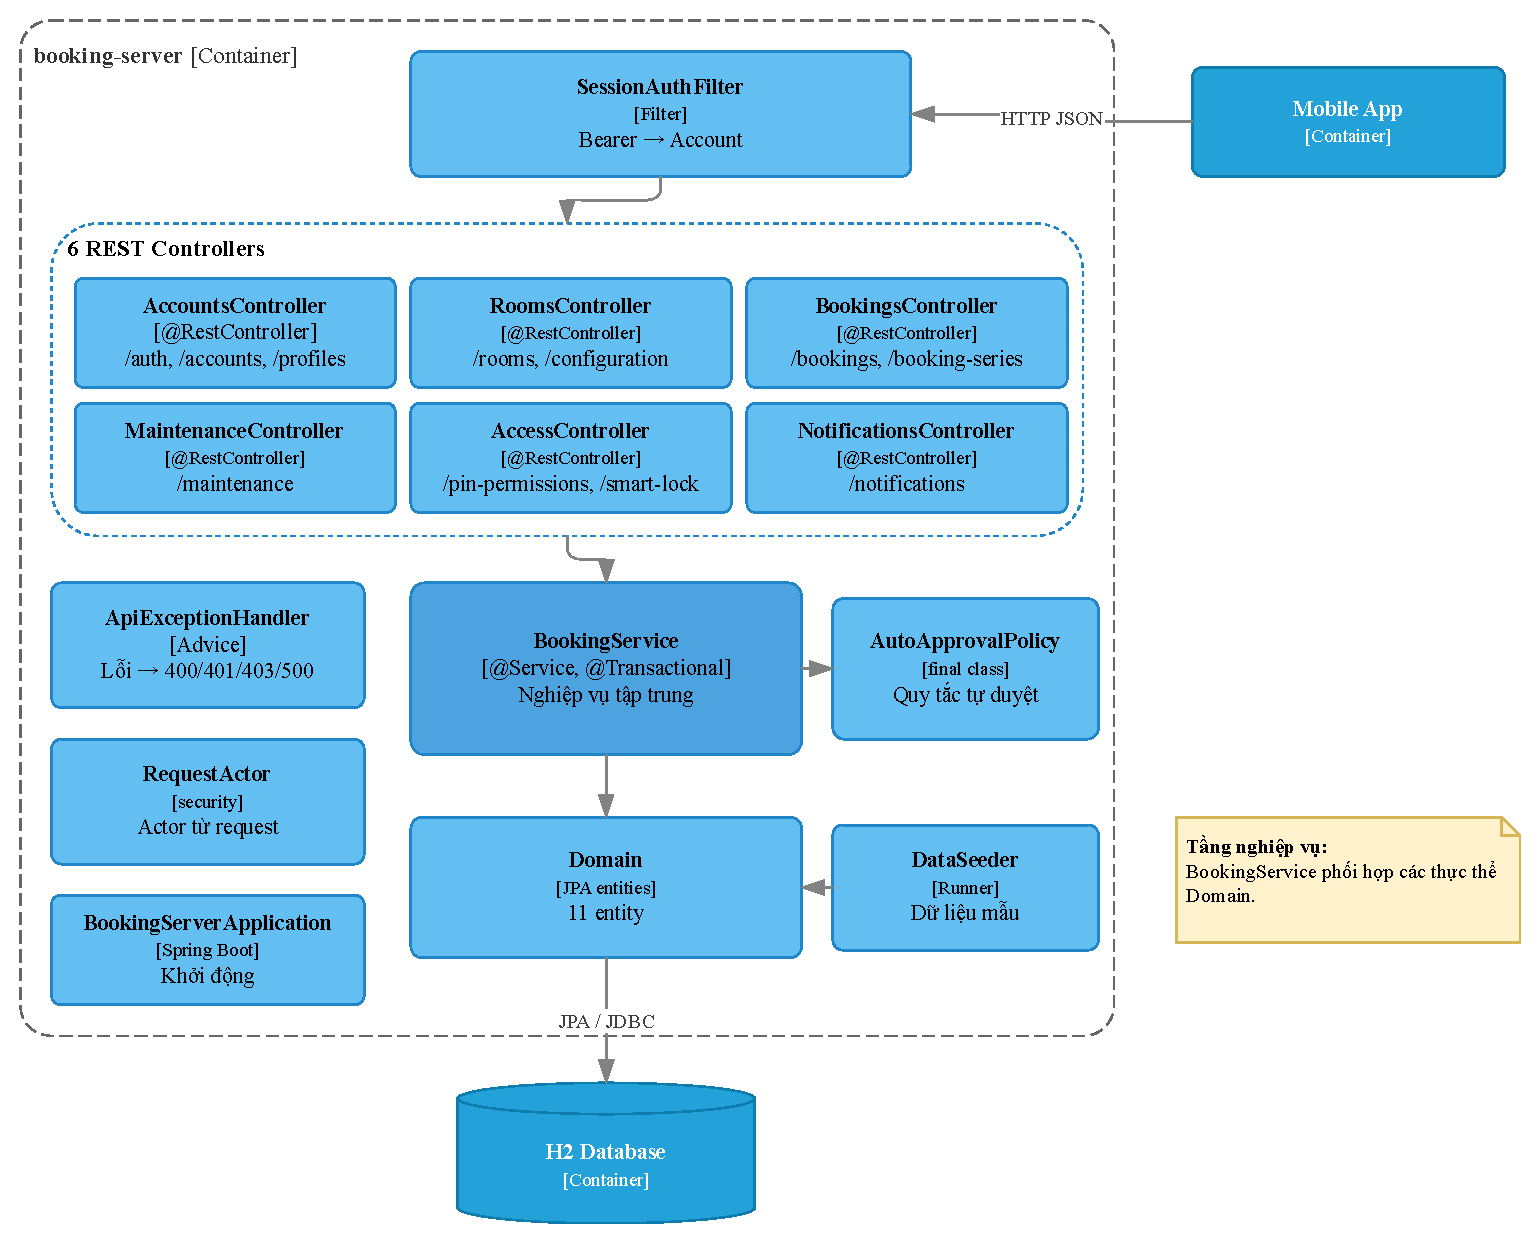
\includegraphics[width=\textwidth,height=.76\textheight,keepaspectratio]{Hinhve/design/12_c4_l3_component_server.pdf}
\caption{Các lớp giao tiếp, nghiệp vụ và lưu trữ của backend}\label{fig:server-components}
\end{figure}

\FloatBarrier
{\tabletext\renewcommand{\arraystretch}{1.04}\begin{longtable}{>{\raggedright\arraybackslash}p{\dimexpr0.28\textwidth-2\tabcolsep\relax}>{\raggedright\arraybackslash}p{\dimexpr0.72\textwidth-2\tabcolsep\relax}}
\caption{Trách nhiệm của 11 module nghiệp vụ}\label{tab:design-modules}\\
\toprule \textbf{Module} & \textbf{Trách nhiệm và cộng tác}\\\midrule
\endfirsthead
\multicolumn{2}{l}{\small Trách nhiệm của 11 module nghiệp vụ (tiếp)}\\
\toprule \textbf{Module} & \textbf{Trách nhiệm và cộng tác}\\\midrule
\endhead
\bottomrule\endlastfoot
\code{auth} & Đăng ký/đăng nhập, mật khẩu và xác thực vai trò; tài khoản quản trị cũng dùng accountRepository.\\\addlinespace[1.5pt]
\code{account_management} & UI quản lý tài khoản và quyền PIN; gọi auth và access control.\\\addlinespace[1.5pt]
\code{room_management} & Danh mục, bộ lọc và sơ đồ tầng; màn tìm và đặt gọi nghiệp vụ booking. Quản lý phòng ghép với bảo trì.\\\addlinespace[1.5pt]
\code{booking} & Tạo, duyệt, lịch lặp, hủy/đổi phòng, nhận chìa, ủy quyền, ghi chú và no-show; dùng phòng, cấu hình, bảo trì, tự duyệt và thông báo.\\\addlinespace[1.5pt]
\code{auto_approval} & Tính quyết định duyệt từ cấu hình và dấu phòng đặc biệt sau khi yêu cầu đã qua validation.\\\addlinespace[1.5pt]
\code{access_control} & Quyền theo user--phòng; tạo và lưu PIN theo booking đã duyệt, gọi smart lock khi có thể gửi.\\\addlinespace[1.5pt]
\code{smart_lock} & Quản lý một khóa gắn phòng; cấp password ID, kết nối native OneIoT và tiếp nhận sự kiện.\\\addlinespace[1.5pt]
\code{schedule_maintenance} & Yêu cầu bảo trì, lịch đã được admin lên và kiểm xung đột.\\\addlinespace[1.5pt]
\code{configuration} & Cửa sổ đặt trước, hạn mức, các thời hạn và công tắc tự duyệt/thông báo.\\\addlinespace[1.5pt]
\code{profile} & Hồ sơ người dùng theo tài khoản.\\\addlinespace[1.5pt]
\code{notifications} & Lưu/đọc theo người nhận, banner và cầu thông báo native; chỉ hiện banner cho tài khoản đang đăng nhập.\\\addlinespace[1.5pt]
\end{longtable}}

Lớp hạ tầng dùng chung cung cấp HTTP client, lưu trữ JSON, cấu hình và xử lý thời gian; lớp giao diện dùng chung cung cấp các thành phần tái sử dụng. Các module cộng tác qua service và hợp đồng dữ liệu, trong đó nghiệp vụ đặt phòng phối hợp với cấu hình, bảo trì, cấp quyền và thông báo.

{\tabletext\renewcommand{\arraystretch}{1.04}\begin{longtable}{>{\raggedright\arraybackslash}p{\dimexpr0.31\textwidth-2\tabcolsep\relax}>{\raggedright\arraybackslash}p{\dimexpr0.69\textwidth-2\tabcolsep\relax}}
\caption{Trách nhiệm các lớp Java và dữ liệu trao đổi}\label{tab:server-responsibilities}\\
\toprule \textbf{Nhóm lớp} & \textbf{Trách nhiệm đã triển khai}\\\midrule
\endfirsthead
\multicolumn{2}{l}{\small Trách nhiệm các lớp Java và dữ liệu trao đổi (tiếp)}\\
\toprule \textbf{Nhóm lớp} & \textbf{Trách nhiệm đã triển khai}\\\midrule
\endhead
\bottomrule\endlastfoot
\code{BookingServerApplication}, \code{DataSeeder} & Khởi động dịch vụ và bổ sung dữ liệu trình diễn, không đại diện cơ sở vật chất thực tế.\\\addlinespace[1.5pt]
\code{SessionAuthFilter}, \code{RequestActor} & Tra token Bearer thành tài khoản, đặt actor trong request và cung cấp actor cho controller.\\\addlinespace[1.5pt]
Sáu controller & Nhận route/body, chuyển actor và dữ liệu tới service, tạo phản hồi HTTP. Các controller dùng chung lớp BookingService.\\\addlinespace[1.5pt]
\code{BookingService} & Xác thực/quyền, các nghiệp vụ và giao dịch; dùng EntityManager để truy vấn, khóa và ghi dữ liệu.\\\addlinespace[1.5pt]
\code{AutoApprovalPolicy} & Quy tắc tự duyệt dùng chung ở luồng tạo booking phía server.\\\addlinespace[1.5pt]
\code{Domain} và converter & 11 entity, cấu trúc nhúng, chuyển danh sách/đối tượng lồng thành JSON.\\\addlinespace[1.5pt]
Record đầu vào/kết quả & Hợp đồng request/response cho phòng, booking, PIN, cấu hình liên quan; tách dữ liệu trao đổi khỏi tham số HTTP.\\\addlinespace[1.5pt]
\code{ApiExceptionHandler} & Chuyển lỗi dữ liệu thành 400, phiên thành 401, quyền thành 403 và lỗi còn lại thành 500, kèm thông điệp JSON.\\\addlinespace[1.5pt]
\end{longtable}}

\subsection{Triển khai trên điện thoại và các kết nối}
Hình~\ref{fig:deployment} mô tả bố trí triển khai: APK/bundle/native chạy trên Android; Java/H2 chạy trên máy chủ; kết nối OneIoT đi từ app tới broker. Metro và ADB phục vụ phát triển hoặc kết nối thử; bản Release local không cần Metro để khởi chạy. Cloudflare và H2 SSL là lựa chọn môi trường, không phải thành phần bắt buộc của bản local.
\begin{figure}[H]\centering
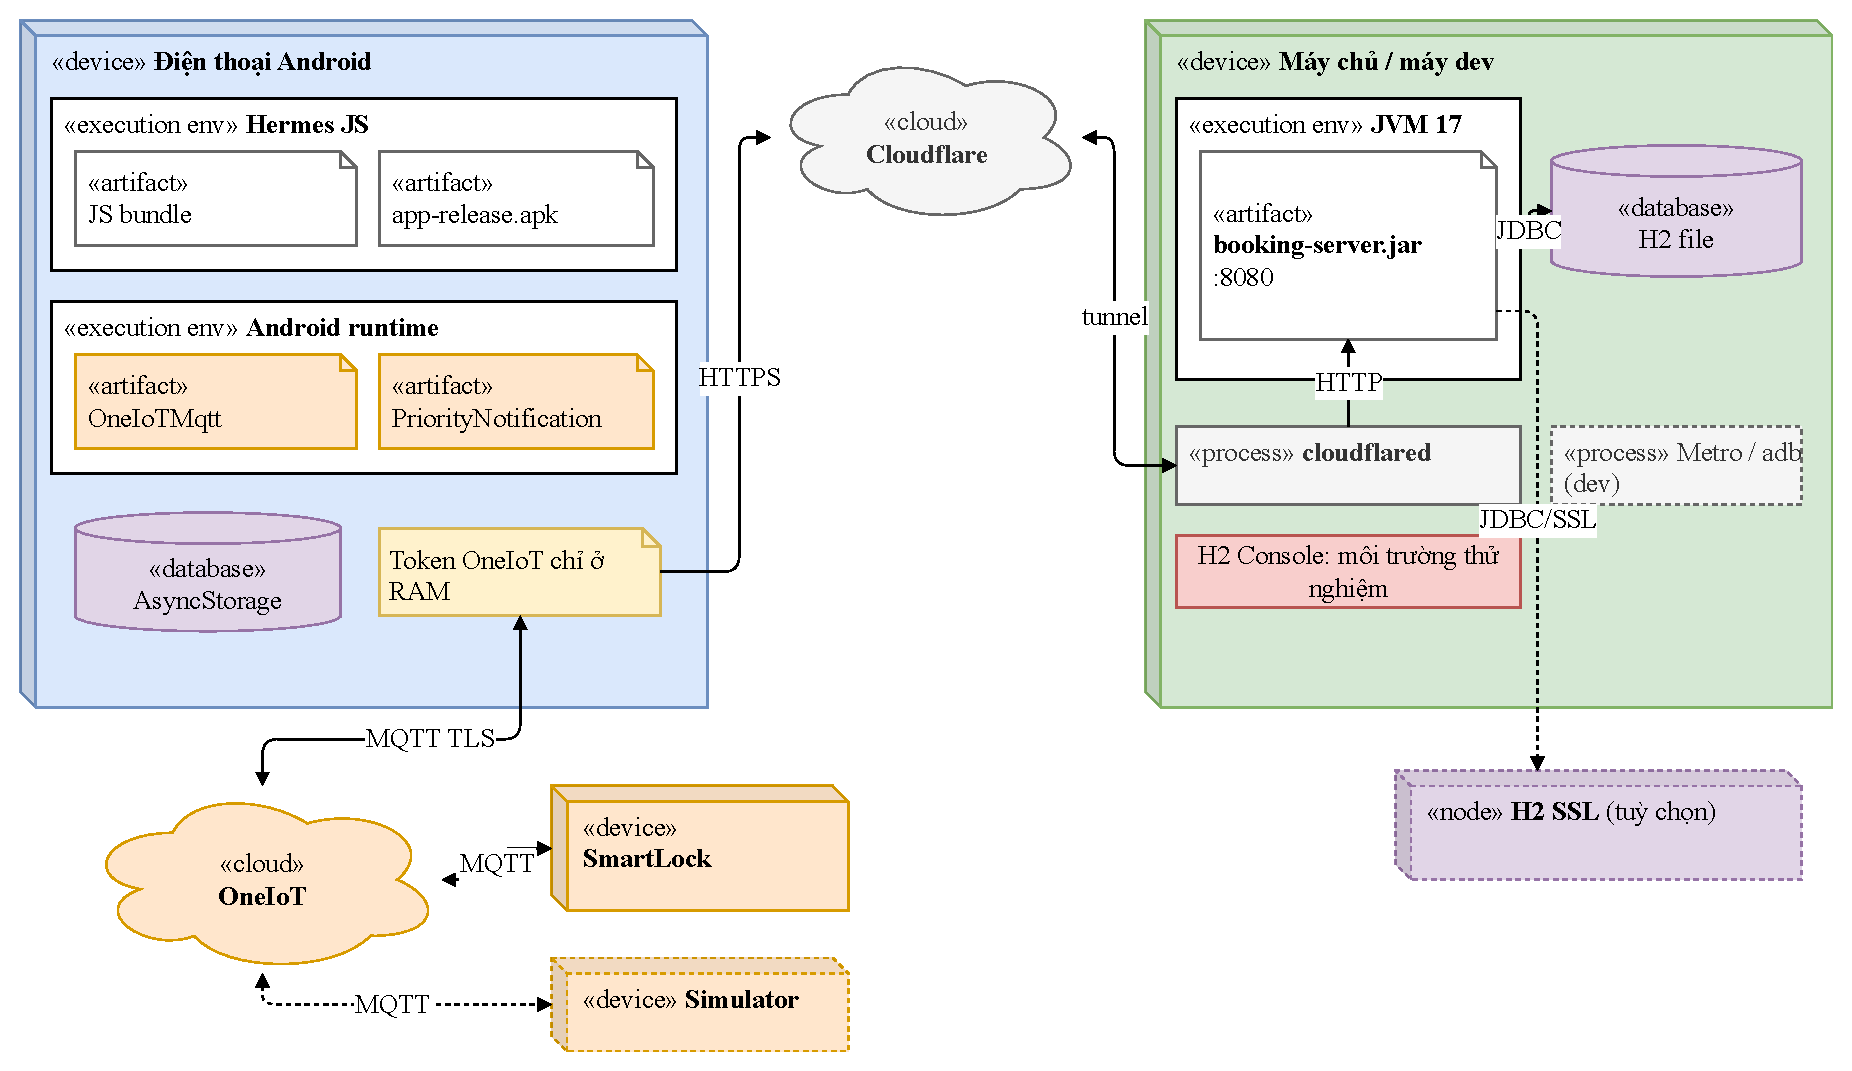
\includegraphics[width=\textwidth,height=.76\textheight,keepaspectratio]{Hinhve/design/14_deployment_diagram.pdf}
\caption{Bố trí triển khai ứng dụng Android, backend và kết nối SmartLock}\label{fig:deployment}
\end{figure}

Ứng dụng Android kết nối trực tiếp OneIoT qua native MQTT để gửi lệnh và tiếp nhận sự kiện từ SmartLock. Backend cung cấp dữ liệu nghiệp vụ qua REST khi bật chế độ remote; chế độ local lưu dữ liệu trên thiết bị. Simulator và gateway là các chương trình hỗ trợ riêng. Các thành phần app và SmartLock đã được nhóm triển khai, chạy thử và hoàn thành các chức năng thực tế.

\FloatBarrier
\section{Mô hình dữ liệu và giao tiếp dịch vụ}
\subsection{Thực thể, thuộc tính và quan hệ logic}
Mô hình dữ liệu gồm tài khoản, tài nguyên phòng và các bản ghi sử dụng, tiếp cận, bảo trì. Các thực thể liên hệ bằng định danh chuỗi; Bảng~\ref{tab:data} tổng hợp thuộc tính và quan hệ chính. Lược đồ ER chi tiết nằm ở Phụ lục~\ref{app:evidence}.
{\tabletext\renewcommand{\arraystretch}{1.04}\begin{longtable}{>{\raggedright\arraybackslash}p{\dimexpr0.27\textwidth-2\tabcolsep\relax}>{\raggedright\arraybackslash}p{\dimexpr0.39\textwidth-2\tabcolsep\relax}>{\raggedright\arraybackslash}p{\dimexpr0.34\textwidth-2\tabcolsep\relax}}
\caption{Mười một thực thể và quan hệ nghiệp vụ chính}\label{tab:data}\\
\toprule \textbf{Thực thể / bảng} & \textbf{Thuộc tính chính} & \textbf{Liên hệ và điều kiện}\\\midrule
\endfirsthead
\multicolumn{3}{l}{\small Mười một thực thể và quan hệ nghiệp vụ chính (tiếp)}\\
\toprule \textbf{Thực thể / bảng} & \textbf{Thuộc tính chính} & \textbf{Liên hệ và điều kiện}\\\midrule
\endhead
\bottomrule\endlastfoot
Account / accounts & username, password, recoveryCode, role, active. & Username là định danh; trạng thái và vai trò quyết định đăng nhập/quyền.\\\addlinespace[1.5pt]
Profile / user\_profiles & username, thông tin họ tên, liên hệ, đơn vị. & Hồ sơ theo tài khoản; user không sửa hồ sơ người khác qua API.\\\addlinespace[1.5pt]
AuthSession / auth\_sessions & token, username, createdAt. & Server tra token để nhận diện actor, không tin username do client tự gửi.\\\addlinespace[1.5pt]
Room / rooms & id, name, floor, capacity, equipment, lockType, status, requiresApproval. & Một phòng có nhiều booking/bảo trì theo thời gian; dấu đặc biệt làm phòng luôn cần admin duyệt.\\\addlinespace[1.5pt]
Booking / bookings & requesterUsername, roomId, date/start/end, purpose, status, metadata duyệt và chuỗi lặp. & Tâm điểm liên kết tài khoản, phòng, PIN, nhận chìa, sự kiện, đổi phòng và yêu cầu bảo trì.\\\addlinespace[1.5pt]
PinPermission / pin\_permissions & username, roomId, active, thông tin cấp/thu hồi. & Quyền cho một cặp tài khoản--phòng, tách khỏi vai trò admin và vẫn phải kiểm booking.\\\addlinespace[1.5pt]
ManagedSmartLock / managed\_smart\_locks & assignedRoomId, thông tin khóa/kết nối, nextPasswordId. & Một khóa quản lý gắn tối đa một phòng PIN; password ID quay vòng 1--255.\\\addlinespace[1.5pt]
Maintenance / maintenance\_records & roomId, date/start/end, reason, cancelledAt. & Lịch hiệu lực chặn khoảng phòng; hủy lịch không xóa lịch sử.\\\addlinespace[1.5pt]
MaintenanceRequest / maintenance\_requests & bookingId, roomId, requesterUsername, reason, status, maintenanceRecordId. & Yêu cầu chờ xử lý khác lịch đã được admin lên.\\\addlinespace[1.5pt]
Notification / notifications & username, title, message, createdAt, read. & Đọc/đánh dấu theo người nhận của phiên.\\\addlinespace[1.5pt]
Configuration / app\_configuration & Cửa sổ ngày, hạn mức, các cutoff/grace, tự duyệt và thông báo. & Bản ghi cấu hình chung được đọc ở các bước kiểm nghiệp vụ.\\\addlinespace[1.5pt]
\end{longtable}}

PIN tạm được nhúng trong Booking bằng \code{@Embedded}; thông tin hẹn/đề xuất nhận chìa, ủy quyền, đổi phòng và danh sách sự kiện dùng cấu trúc lồng hoặc converter JSON. Các quan hệ trên ERD biểu diễn tham chiếu logic theo định danh; tính hợp lệ của các liên hệ được kiểm ở tầng nghiệp vụ, thay cho ánh xạ toàn bộ bằng quan hệ đối tượng JPA.

Dữ liệu thời gian trao đổi gồm ngày dạng YYYY-MM-DD, giờ HH:mm và các mốc ISO/epoch tùy trường. Service Java dùng múi giờ Việt Nam khi kiểm nghiệp vụ, còn local dựng thời điểm theo thiết bị. Đồng hồ và múi giờ ảnh hưởng trực tiếp đến đặt cùng ngày, no-show và khoảng hiệu lực PIN.

\subsection{Hợp đồng REST và xử lý lỗi}
Giao tiếp REST được tổ chức theo sáu controller nghiệp vụ. Các nhóm API bao gồm tài khoản, phòng, booking, lịch lặp, quyền truy cập, nhận chìa, điểm danh, bảo trì và thông báo. Bảng~\ref{tab:api-design} tổng hợp 51 cặp phương thức/đường dẫn thành 20 nhóm thao tác.
{\tabletext\renewcommand{\arraystretch}{1.04}\begin{longtable}{>{\raggedright\arraybackslash}p{\dimexpr0.49\textwidth-2\tabcolsep\relax}>{\raggedright\arraybackslash}p{\dimexpr0.51\textwidth-2\tabcolsep\relax}}
\caption{Tổng hợp endpoint, dữ liệu và quyền truy cập}\label{tab:api-design}\\
\toprule \textbf{Phương thức / đường dẫn} & \textbf{Dữ liệu và kiểm soát}\\\midrule
\endfirsthead
\multicolumn{2}{l}{\small Tổng hợp endpoint, dữ liệu và quyền truy cập (tiếp)}\\
\toprule \textbf{Phương thức / đường dẫn} & \textbf{Dữ liệu và kiểm soát}\\\midrule
\endhead
\bottomrule\endlastfoot
\code{POST /api/auth/login}; \code{POST /api/auth/register} & Login nhận username/password, trả token/username/role. Đăng ký kiểm dữ liệu và trả phiên; không cần token trước.\\\addlinespace[1.5pt]
\code{POST /api/auth/change-password}; \code{POST /api/auth/reset-password} & Đổi mật khẩu dùng actor/mật khẩu hiện tại; reset dùng username/mã khôi phục. Reset là ngoại lệ không bắt token tại filter.\\\addlinespace[1.5pt]
\code{GET,POST /api/accounts}; \code{PUT,DELETE /api/accounts/{username}} & Admin quản lý tài khoản; service chặn các thao tác vi phạm quyền hoặc điều kiện dữ liệu đang dùng.\\\addlinespace[1.5pt]
\code{GET,PUT /api/profiles/{username}} & Hồ sơ gắn tài khoản; service kiểm quyền truy cập theo actor.\\\addlinespace[1.5pt]
\code{GET,POST /api/rooms}; \code{PUT,DELETE /api/rooms/{id}} & Danh sách cho phiên hợp lệ; ghi phòng cần admin, kiểm tên/tầng/sức chứa/loại khóa.\\\addlinespace[1.5pt]
\code{GET,PUT /api/configuration} & Đọc quy tắc; admin ghi. Client cũ bỏ qua trường mới không làm mất giá trị hiện có theo code xử lý.\\\addlinespace[1.5pt]
\code{GET /api/room-occupancy} & Trả các khoảng sử dụng để tính trạng thái phòng theo lịch, không chỉ theo cờ AVAILABLE.\\\addlinespace[1.5pt]
\code{GET,POST /api/bookings} & Đọc theo phạm vi tài khoản; tạo nhận phòng/ngày/giờ/mục đích/lặp, kiểm role và quy tắc trước ghi.\\\addlinespace[1.5pt]
\code{POST /api/bookings/{id}/review}; \code{POST /api/bookings/{id}/change-room} & Admin duyệt/từ chối hoặc đổi phòng; kiểm trạng thái, quyền và điều kiện áp dụng.\\\addlinespace[1.5pt]
\code{POST /api/bookings/{id}/cancel} & User chủ lượt; kiểm trạng thái/thời hạn, chuyển CANCELLED và đánh dấu PIN thu hồi trong dữ liệu; không xóa quyền phòng toàn cục.\\\addlinespace[1.5pt]
\code{POST /api/booking-series/{seriesId}/review}; \code{PUT /api/booking-series/{seriesId}/pending}; \code{POST /api/booking-series/{seriesId}/cancel} & Xử lý các lượt trong chuỗi theo trạng thái; không xem thao tác chuỗi là quyền bỏ qua xung đột từng lượt.\\\addlinespace[1.5pt]
\code{GET,POST /api/pin-permissions}; \code{POST /api/pin-permissions/revoke} & Đọc/cấp/thu hồi quyền theo user--phòng; thao tác quản trị kiểm role trong service.\\\addlinespace[1.5pt]
\code{POST /api/bookings/{id}/temporary-pin} & Lưu/cập nhật mã, khoảng hiệu lực và trạng thái gửi; kiểm chủ lượt/admin, booking đã duyệt và quyền liên quan.\\\addlinespace[1.5pt]
\code{GET /api/smart-lock}; \code{POST /api/smart-lock/assign}; \code{POST /api/smart-lock/unassign}; \code{POST /api/smart-lock/reserve-password-id} & Quản lý khóa/phòng và cấp ID; cấp ID kiểm phòng khớp, khóa dữ liệu và quyền user nếu actor không phải admin.\\\addlinespace[1.5pt]
\code{POST /api/bookings/{id}/pickup/propose}; \code{POST /api/bookings/{id}/pickup/schedule}; \code{POST /api/bookings/{id}/pickup/accept}; \code{PUT /api/bookings/{id}/delegate} & Trao đổi thời gian/địa điểm nhận chìa và người nhận hộ; service kiểm quyền và thứ tự trạng thái thương lượng.\\\addlinespace[1.5pt]
\code{POST /api/bookings/access-event}; \code{POST /api/bookings/{id}/check-in}; \code{POST /api/bookings/{id}/no-show} & Ghi sự kiện khóa hoặc xác nhận điểm danh theo quyền; kiểm thời gian và bằng chứng có mặt/no-show.\\\addlinespace[1.5pt]
\code{GET,POST /api/maintenance}; \code{POST /api/maintenance/{id}/cancel} & Đọc/lập/hủy lịch bảo trì; lập lịch cần admin và kiểm xung đột.\\\addlinespace[1.5pt]
\code{GET,POST /api/maintenance/requests}; \code{POST /api/maintenance/requests/{id}/schedule}; \code{POST /api/maintenance/requests/{id}/reject} & Yêu cầu từ booking đang dùng, được admin lên lịch hoặc từ chối.\\\addlinespace[1.5pt]
\code{POST /api/bookings/{id}/room-observation} & Gửi ghi chú cho admin, không tự tạo yêu cầu hoặc lịch bảo trì.\\\addlinespace[1.5pt]
\code{GET,POST /api/notifications}; \code{POST /api/notifications/read} & Đọc/đánh dấu theo phiên; tạo thông báo còn phải qua kiểm tra quyền service.\\\addlinespace[1.5pt]
\end{longtable}}

\code{SessionAuthFilter} bỏ qua ba route login/register/reset-password; các route API còn lại cần token Bearer hợp lệ. User không được chọn username người khác để mở rộng dữ liệu trả về. Client bọc fetch, thêm Authorization, xử lý JSON/204/401 và timeout 12 giây; API lỗi dùng trường \textit{\{message\}}. Kết quả kiểm thử API và tích hợp được trình bày ở Chương~\ref{chap:testing}.

\FloatBarrier
\section{Thiết kế giao diện và điều hướng}
\subsection{Luồng màn hình theo vai trò}
Giao diện Android dọc dùng dashboard, đầu trang, Back, chuông và menu tài khoản. Tìm phòng theo tầng/ngày/giờ và gửi yêu cầu trên cùng màn hình. Hình~\ref{fig:flow-user}--\ref{fig:flow-admin} mô tả điều hướng hai vai trò; ảnh thực nghiệm ở Chương~\ref{chap:implementation}.
\begin{figure}[H]\centering
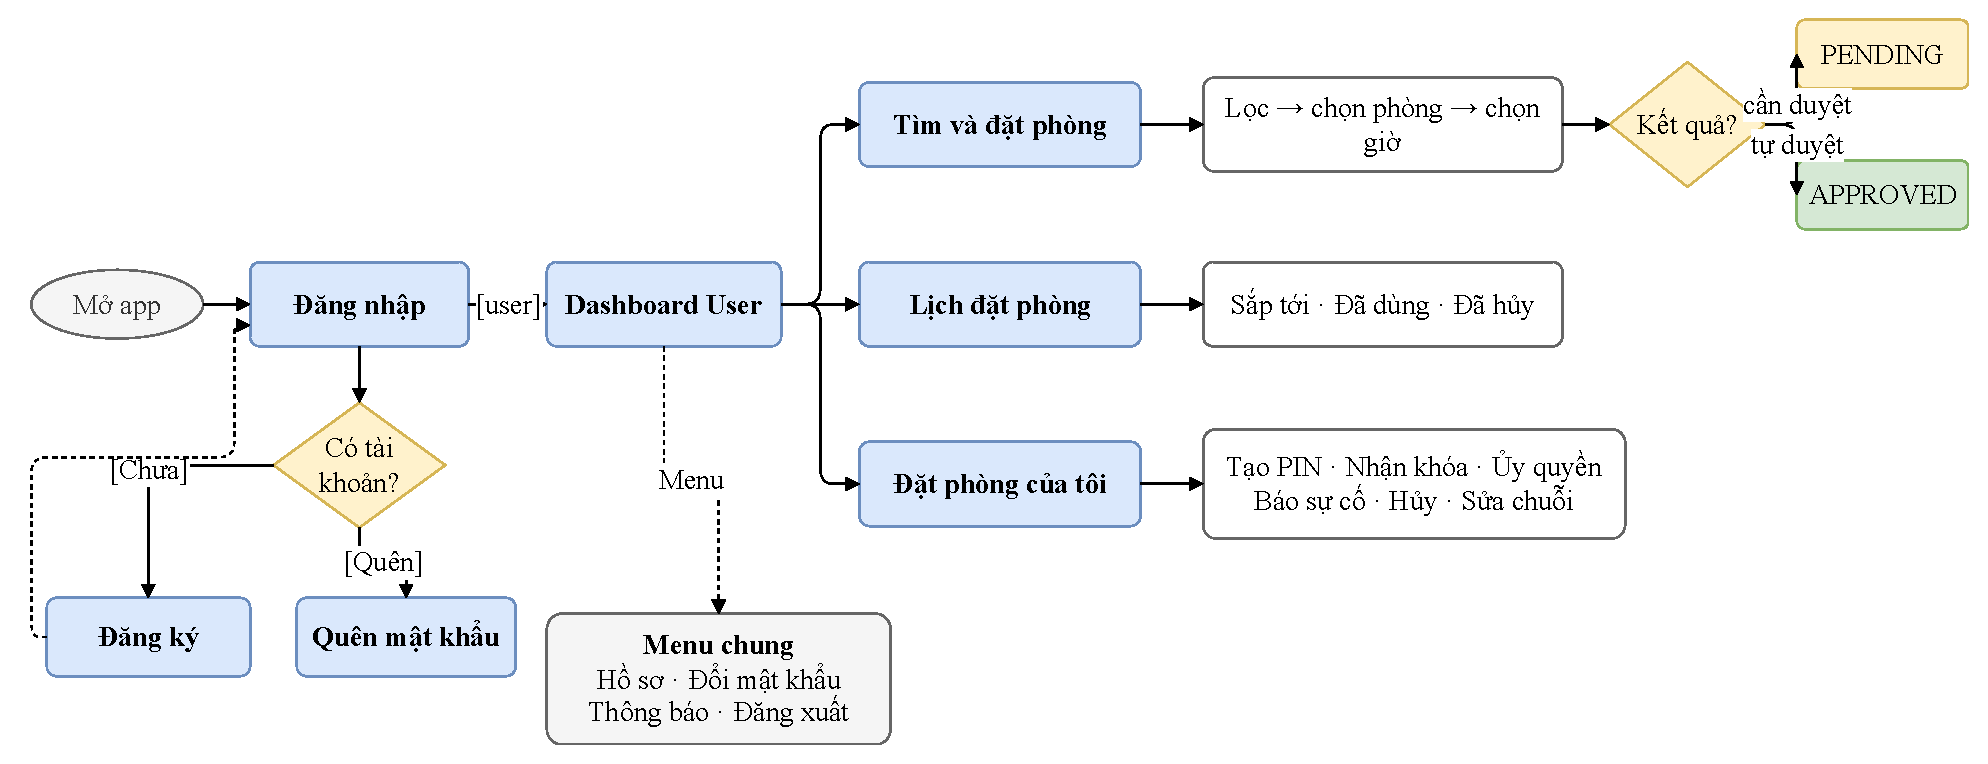
\includegraphics[width=\textwidth,height=.76\textheight,keepaspectratio]{Hinhve/design/05a_user_flow_nguoi_dung.pdf}
\caption{Luồng màn hình và các tác vụ chính của người dùng}\label{fig:flow-user}
\end{figure}
\begin{figure}[H]\centering
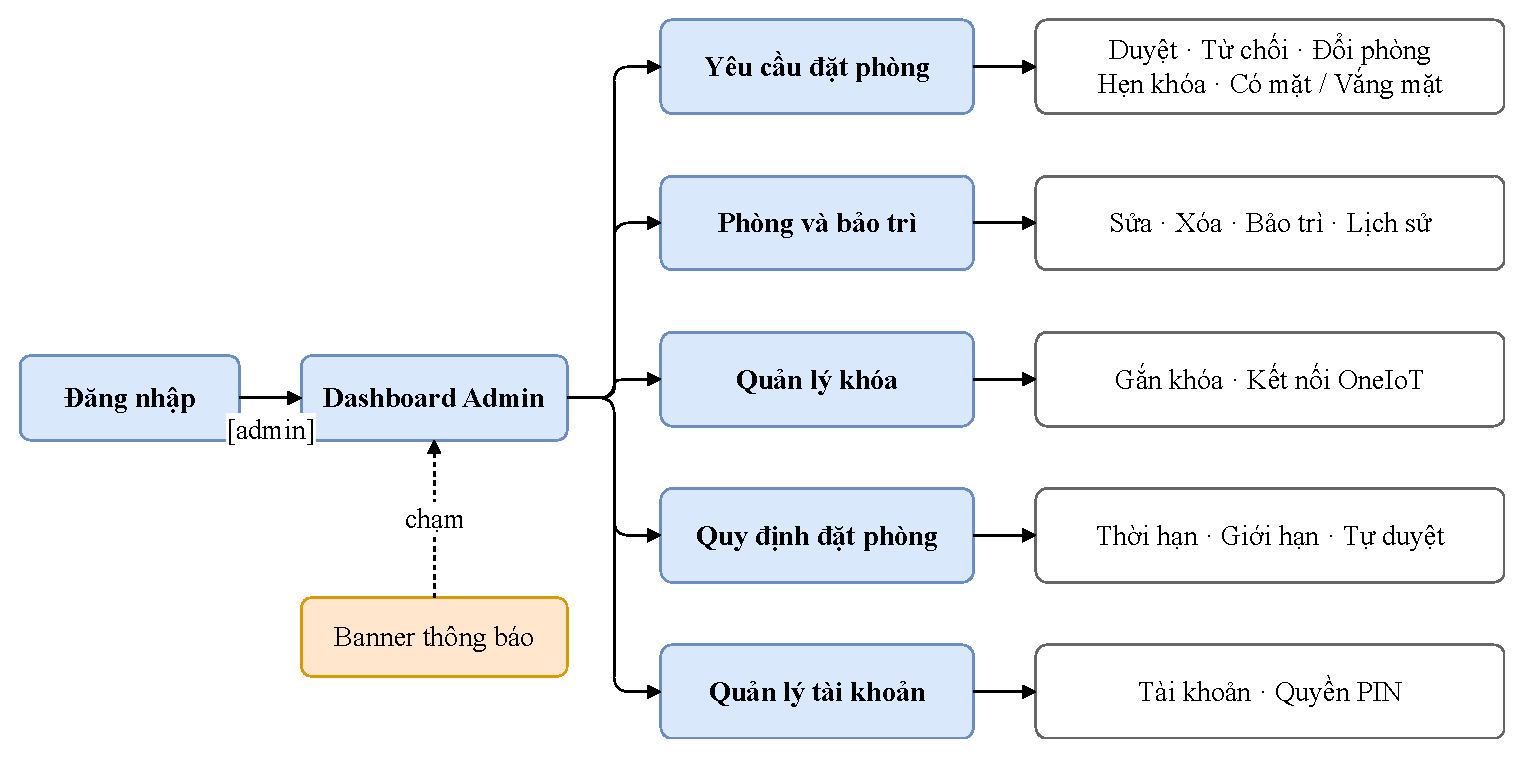
\includegraphics[width=\textwidth,height=.76\textheight,keepaspectratio]{Hinhve/design/05b_user_flow_quan_tri_vien.pdf}
\caption{Luồng màn hình quản trị và các điểm vào từ thông báo}\label{fig:flow-admin}
\end{figure}

\FloatBarrier
{\tabletext\renewcommand{\arraystretch}{1.04}\begin{longtable}{>{\raggedright\arraybackslash}p{\dimexpr0.31\textwidth-2\tabcolsep\relax}>{\raggedright\arraybackslash}p{\dimexpr0.69\textwidth-2\tabcolsep\relax}}
\caption{Màn hình, mục đích và dữ liệu điều hướng}\label{tab:navigation}\\
\toprule \textbf{Điểm vào} & \textbf{Trách nhiệm / tham số}\\\midrule
\endfirsthead
\multicolumn{2}{l}{\small Màn hình, mục đích và dữ liệu điều hướng (tiếp)}\\
\toprule \textbf{Điểm vào} & \textbf{Trách nhiệm / tham số}\\\midrule
\endhead
\bottomrule\endlastfoot
Đăng nhập, đăng ký, khôi phục mật khẩu & Chọn form xác thực qua selectedFeature trong LoginScreen; khi đăng nhập thành công, callback chuyển session lên App.\\\addlinespace[1.5pt]
Dashboard User & Mở Tìm và đặt phòng, Lịch đặt phòng, Đặt phòng của tôi; truyền username và onBack cho màn con.\\\addlinespace[1.5pt]
Dashboard Admin & Mở Yêu cầu đặt phòng, Quản lý tài khoản, Quản lý phòng và bảo trì, Quản lý khóa, Quy định đặt phòng; truyền thông tin admin khi cần.\\\addlinespace[1.5pt]
Menu tài khoản và chuông & Mở hồ sơ, đổi mật khẩu, thông báo; logout xóa phiên trong UI. Banner/notification có thể đưa admin tới màn xử lý yêu cầu.\\\addlinespace[1.5pt]
Đặt phòng của tôi & Phân nhóm lượt theo thời gian/trạng thái; mở thao tác sửa/hủy chuỗi, PIN, nhận chìa, ủy quyền và phản ánh phòng.\\\addlinespace[1.5pt]
Quản lý phòng và bảo trì & Chọn tầng/phòng; chỉnh thông tin, xem lịch hoặc lập/xử lý bảo trì trên cùng màn hình.\\\addlinespace[1.5pt]
\end{longtable}}

\subsection{Cơ chế chuyển màn, làm mới và quay lại}
Bảng điều khiển dùng trạng thái \code{activeScreen} để chọn màn hình hiển thị. Props mang dữ liệu và callback thay route params. Khi đóng màn con, \code{closeChildScreen} đặt màn đang chọn về null rồi làm mới số thông báo/yêu cầu. BackHandler đóng menu trước, sau đó quay về dashboard; listener được tháo khi effect thay đổi hoặc unmount.

App yêu cầu đăng nhập lại khi khởi động; các màn hình được điều khiển bằng state và callback. Loading/error và cleanup listener/timer là trách nhiệm từng luồng bất đồng bộ.

\FloatBarrier
\section{Dữ liệu cá nhân, quyền thiết bị và các ràng buộc}
AndroidManifest khai báo INTERNET, POST\_NOTIFICATIONS và VIBRATE. Trên Android từ API 33, app kiểm và xin quyền thông báo khi chạy \cite{android}; từ chối quyền không đồng nghĩa nghiệp vụ đặt phòng bị cấm, nhưng thông báo hệ điều hành có thể không hiện. Ứng dụng không xin quyền vị trí, camera hoặc micro cho luồng đặt phòng hiện tại.

Token REST và OneIoT giữ trong RAM của phiên. Token OneIoT không được ghi vào source hoặc Async Storage; app ngắt MQTT khi đăng xuất hoặc xuống nền, việc nhận sự kiện khóa diễn ra trong phiên MQTT đang hoạt động. Mật khẩu/PIN và một phần dữ liệu khôi phục hiện còn dạng rõ trong local/entity server. Mã hóa gói lệnh khóa không giải quyết việc bảo vệ các dữ liệu lưu này.

Native TLS đang bỏ qua xác minh chứng thư; Android cho phép cleartext để thử HTTP. Hướng gia cố bảo mật gồm xác thực, bảo vệ lưu trữ, chứng thư và phân quyền khi mở rộng triển khai. H2 console và đường tunnel trong sơ đồ là cấu hình thử nghiệm cần quản lý theo môi trường. Chế độ local dùng được khi thiếu backend, nhưng đó là chế độ chọn trước khi build, không phải cơ chế tự fallback/offline sync của REST.

\FloatBarrier
\section{Các giải pháp kỹ thuật cho luồng nghiệp vụ cốt lõi}
Ba nhóm giải pháp tập trung vào tính nhất quán lịch, quyền tiếp cận và tổ chức dữ liệu. Chúng giải thích cách các bước kiểm tra, trạng thái và ranh giới dữ liệu hỗ trợ luồng nghiệp vụ cốt lõi.

\subsection{Chống trùng lịch, giao dịch và quyết định duyệt}
\label{sec:overlap-solution}
\paragraph{Bài toán.} Hai lượt đặt có thể không trùng khi đọc riêng nhưng xung đột khi cùng được ghi. Cần phân biệt khoảng chạm biên với khoảng giao nhau; đồng thời kiểm lại phòng khi admin duyệt vì lịch bảo trì hoặc lượt đã duyệt có thể thay đổi trong thời gian chờ.

\paragraph{Phép kiểm khoảng.} Với cùng ngày, hai khoảng nửa mở \textit{[s1,e1)} và \textit{[s2,e2)} giao nhau khi đồng thời có \textit{s1 < e2} và \textit{s2 < e1}. Dùng bất đẳng thức chặt nên 08:00--09:00 và 09:00--10:00 được xem là liền kề. Ngày khác nhau không giao trong phép kiểm này. Dữ liệu thời gian được chuẩn hóa và kiểm tra trước phép so sánh; khoảng có giờ bắt đầu lớn hơn hoặc bằng giờ kết thúc bị từ chối.

Nghiệp vụ đặt phòng và bảo trì dùng chung phép kiểm khoảng; backend thực hiện điều kiện tương ứng trong tầng dịch vụ. Khi tạo, hệ thống xét phòng, lịch của chính user và bảo trì; khi duyệt một lượt đang chờ, code kiểm lại thời gian kết thúc, bảo trì và xung đột với lượt đã duyệt của phòng. Kiểm tra khi tạo bảo đảm yêu cầu hợp lệ; kiểm tra khi duyệt bảo đảm quyết định dựa trên lịch và bảo trì hiện thời.

\paragraph{Thứ tự giao dịch ở backend.} \code{BookingService.createBooking} dùng \code{@Transactional}, khóa Configuration và Room bằng \code{PESSIMISTIC_WRITE} trước khi đọc lịch. Với chuỗi lặp, từng lượt được sinh, kiểm và bổ sung vào tập xét để phát hiện cả xung đột trong chuỗi (Bảng~\ref{tab:create-transaction}).
{\tabletext\renewcommand{\arraystretch}{1.04}\begin{longtable}{>{\raggedright\arraybackslash}p{\dimexpr0.12\textwidth-2\tabcolsep\relax}>{\raggedright\arraybackslash}p{\dimexpr0.88\textwidth-2\tabcolsep\relax}}
\caption{Thứ tự tạo booking trong giao dịch Java}\label{tab:create-transaction}\\
\toprule \textbf{Bước} & \textbf{Xử lý}\\\midrule
\endfirsthead
\multicolumn{2}{l}{\small Thứ tự tạo booking trong giao dịch Java (tiếp)}\\
\toprule \textbf{Bước} & \textbf{Xử lý}\\\midrule
\endhead
\bottomrule\endlastfoot
1 & Kiểm actor là user và không mạo danh requesterUsername khác.\\\addlinespace[1.5pt]
2 & Khóa cấu hình chung và bản ghi phòng được chọn trước khi đọc lịch.\\\addlinespace[1.5pt]
3 & Kiểm định dạng ngày và số tuần lặp; sinh ngày của từng lượt nếu đặt theo chuỗi.\\\addlinespace[1.5pt]
4 & Validate từng lượt: phòng, giờ, bảo trì, chồng phòng/user, mục đích, cửa sổ và hạn mức theo điều kiện của lượt đầu/lượt lặp.\\\addlinespace[1.5pt]
5 & Tạo booking với trạng thái ban đầu PENDING; lưu metadata chuỗi và bổ sung vào tập đang xét.\\\addlinespace[1.5pt]
6 & Sau validation, AutoApprovalPolicy quyết định có tự duyệt: chỉ khi công tắc bật và phòng không yêu cầu duyệt riêng.\\\addlinespace[1.5pt]
7 & Nhánh tự duyệt cập nhật APPROVED, người duyệt system, quyền PIN nếu phòng PIN và thông báo; nhánh thủ công giữ PENDING và báo admin.\\\addlinespace[1.5pt]
8 & Trả BookingResult trong giao dịch. Lỗi dữ liệu/điều kiện được ném thành ngoại lệ; không trả kết quả thành công cho lượt vi phạm.\\\addlinespace[1.5pt]
\end{longtable}}

\code{reviewBooking} khóa Configuration và booking đích; khi duyệt sẽ kiểm trạng thái PENDING và các điều kiện hiện thời rồi cập nhật quyết định. Quyền PIN được cấp cho phòng khóa số sau khi duyệt. Sơ đồ trình tự Hình~\ref{fig:sequence-booking} bổ sung điểm gọi qua UI, client HTTP, filter, controller và service; thứ tự khóa và kiểm tra dữ liệu được tổng hợp trong Bảng~\ref{tab:create-transaction}.
\begin{figure}[H]\centering
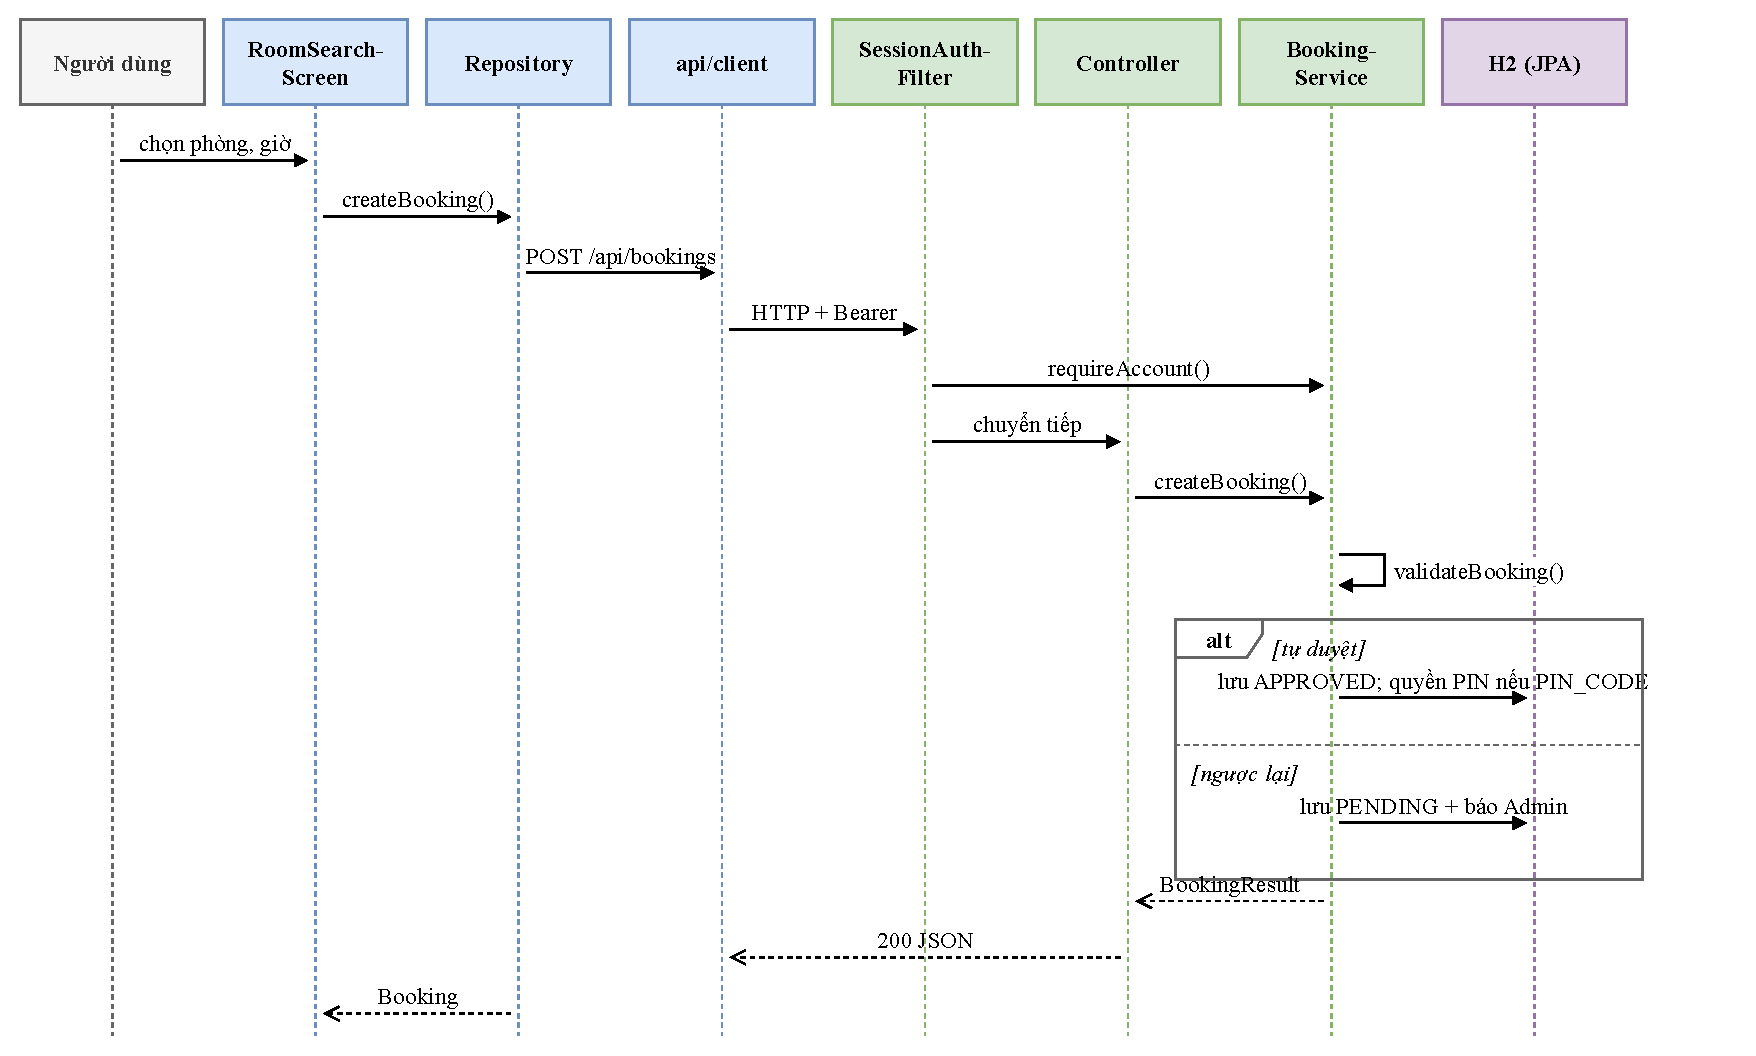
\includegraphics[width=\textwidth,height=.76\textheight,keepaspectratio]{Hinhve/design/15b_sequence_tao_yeu_cau_dat_phong.pdf}
\caption{Trình tự tạo booking qua REST và nhánh tự duyệt/thủ công}\label{fig:sequence-booking}
\end{figure}

\paragraph{Kết quả và hạn chế kỹ thuật.} Các ca kiểm thử ở Chương~\ref{chap:testing} xác nhận xử lý đúng trùng lịch, chạm biên, bảo trì và hạn mức. Backend khóa bản ghi cấu hình/phòng trước khi kiểm và ghi dữ liệu. Khóa cấu hình chung khiến các thao tác dùng cùng tài nguyên phải chờ nhau, là điểm cần tối ưu khi mở rộng. Kho local đọc/ghi JSON, còn backend quản lý giao dịch và khóa dữ liệu bằng JPA.

\FloatBarrier
\subsection{Cấp quyền theo phòng và vòng đời PIN tạm thời}
\label{sec:pin-solution}
\paragraph{Bài toán.} Vai trò user không được biến thành quyền tạo mã ở mọi phòng. Một người chỉ được tạo PIN cho booking đã duyệt của mình, tại phòng được phép và đang gắn khóa phù hợp. Kết nối OneIoT có thể chưa có khi tạo mã, vì vậy lưu mã và gửi lệnh cần là các trạng thái riêng.

\paragraph{Kiểm quyền ở các tầng.} Dịch vụ cấp PIN kiểm vai trò, booking tồn tại/APPROVED, phòng PIN, chủ lượt/quyền theo phòng đối với user, chưa có PIN chưa thu hồi và lượt chưa kết thúc. Admin có quyền thao tác phù hợp nhưng vẫn phải đáp ứng các điều kiện nghiệp vụ của booking/phòng. Khi duyệt tay hoặc tự duyệt phòng PIN, hệ thống cấp quyền cho cặp username--roomId. Thu hồi quyền theo phòng tách khỏi thay đổi role tài khoản.

Mã mới chỉ được tạo khi lượt đặt không còn PIN chưa thu hồi. Do đó, PIN hết thời gian nhưng chưa ghi nhận thu hồi vẫn ngăn việc cấp mã tiếp theo.

\paragraph{Khoảng hiệu lực và ID khóa.} Mã nghiệp vụ có đúng bảy chữ số. Với khoảng sử dụng, validFrom được tính bằng giờ bắt đầu trừ khoảng đệm; validUntil bằng giờ kết thúc cộng khoảng đệm. Giá trị mặc định là 10 phút và đọc từ cấu hình, không gắn cứng trong UI. Trước khi lưu, service xin password ID của khóa gắn phòng; ID nằm trong 1--255 và quay vòng sau 255. Backend khóa bản ghi khóa khi cấp ID. Cấp ID, lưu PIN và gửi MQTT là các lời gọi riêng trong quy trình.

\paragraph{Lưu trước, gửi khi có phiên.} App lưu code, thời hạn và password ID vào booking trước. Nếu OneIoT chưa nối, người dùng vẫn xem được mã và trạng thái chờ. Khi có phiên, \code{deliverPendingTemporaryPins} duyệt các PIN chưa thu hồi/chưa gửi, booking còn APPROVED, đúng phòng đang gắn khóa và chưa hết hạn. Một lần gửi thất bại được ghi thông tin lần thử/lỗi để UI phân biệt với chưa thử gửi.

\begin{figure}[H]\centering
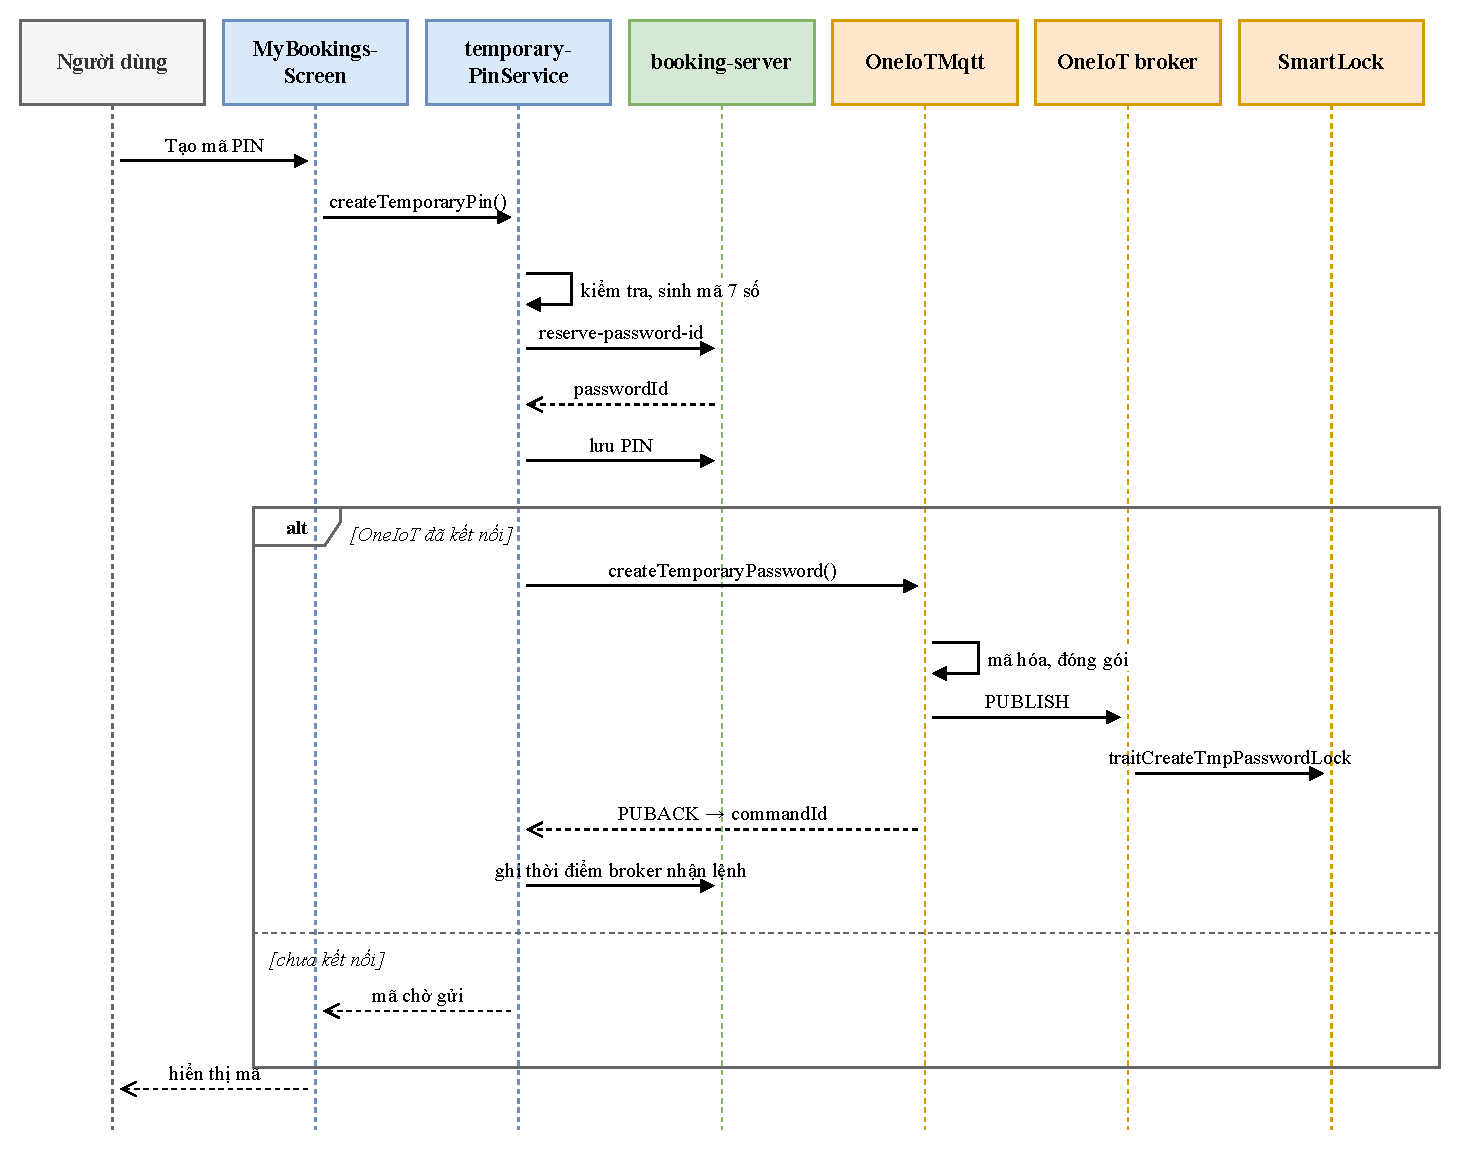
\includegraphics[width=\textwidth,height=.76\textheight,keepaspectratio]{Hinhve/design/16a_sequence_tao_pin_tam.pdf}
\caption{Tạo, lưu và gửi PIN; xác nhận publish của broker tách với thực thi trên khóa}\label{fig:sequence-pin}
\end{figure}

Native \code{OneIoTMqttPackage.kt} chuyển thời hạn sang định dạng bản tin, mã hóa phần mật khẩu và gửi trait \code{traitCreateTmpPasswordLock}. Sau publish được broker xác nhận, app lưu \code{lockDeliveredAt} và request ID. Giao diện cập nhật trạng thái gửi theo kết quả publish; các bản tin sự kiện khóa được xử lý qua luồng nhận MQTT.

\paragraph{Kết quả và hạn chế kỹ thuật.} Các kiểm thử access control và native bridge xác nhận đúng dữ liệu, quyền, thời hạn và cơ chế gửi lại. Ứng dụng và SmartLock thực hiện luồng cấp, sử dụng PIN thực tế. Trạng thái revokedAt quản lý PIN trong booking. Hướng gia cố gồm quản lý ID hữu hạn, bảo vệ dữ liệu, nguồn sinh mã và phản hồi thiết bị.

\FloatBarrier
\subsection{Cùng giao diện nghiệp vụ, hai chế độ dữ liệu}
\label{sec:two-data-solution}
\paragraph{Bài toán.} Hệ thống hỗ trợ vận hành độc lập trên một thiết bị và sử dụng dữ liệu dùng chung qua REST. Hai chế độ dùng cùng giao diện nghiệp vụ để giảm lặp xử lý; nguồn dữ liệu được chọn rõ ràng trong cấu hình bản build.

\paragraph{Giải pháp triển khai.} Repository giữ các hàm nghiệp vụ mà UI gọi; \code{isRemoteApiEnabled} chọn nhánh REST hoặc đọc/ghi JSON local. Client tập trung thêm token và chuyển lỗi mạng/HTTP thành Error cho màn hình. Kiểu TypeScript và cấu trúc request/response Java xác định hợp đồng trao đổi; kiểm thử API kiểm tra phương thức, dữ liệu, phiên và các nhánh lỗi.
{\tabletext\renewcommand{\arraystretch}{1.04}\begin{longtable}{>{\raggedright\arraybackslash}p{\dimexpr0.22\textwidth-2\tabcolsep\relax}>{\raggedright\arraybackslash}p{\dimexpr0.37\textwidth-2\tabcolsep\relax}>{\raggedright\arraybackslash}p{\dimexpr0.41\textwidth-2\tabcolsep\relax}}
\caption{Đối chiếu thao tác local và REST}\label{tab:local-remote}\\
\toprule \textbf{Thao tác} & \textbf{Local} & \textbf{REST}\\\midrule
\endfirsthead
\multicolumn{3}{l}{\small Đối chiếu thao tác local và REST (tiếp)}\\
\toprule \textbf{Thao tác} & \textbf{Local} & \textbf{REST}\\\midrule
\endhead
\bottomrule\endlastfoot
Xác thực & Đọc tài khoản của kho thiết bị, tạo session UI. & Login tạo token/actor tại server; request sau mang Bearer.\\\addlinespace[1.5pt]
Tạo/duyệt booking & Repository kiểm quy tắc trên các tập dữ liệu local và ghi JSON. & API/service kiểm actor và dữ liệu trong giao dịch; server là nơi quyết định trạng thái được lưu.\\\addlinespace[1.5pt]
Phòng/cấu hình/bảo trì & Mỗi máy giữ danh mục và cấu hình riêng. & Các client gọi cùng server sử dụng chung danh mục, cấu hình và dữ liệu phòng.\\\addlinespace[1.5pt]
Quyền và PIN & Quyền và PIN gắn tài khoản/phòng/booking trong kho local. & Quyền và PIN lưu ở server; việc gửi MQTT vẫn xuất phát từ app/native, không chuyển cho Java.\\\addlinespace[1.5pt]
Thông báo & Lưu theo người nhận trong thiết bị; banner chỉ hiện cho tài khoản đang đăng nhập. & Server lưu theo user; client tải thông báo qua REST bằng phiên đăng nhập.\\\addlinespace[1.5pt]
Lỗi kết nối & Không cần booking server; OneIoT vẫn là kết nối riêng nếu dùng khóa. & Trả lỗi/timeout theo client; không tự fallback hoặc tải backlog local.\\\addlinespace[1.5pt]
\end{longtable}}

\paragraph{Kết quả và hạn chế kỹ thuật.} Một nhóm màn hình phục vụ cả hai chế độ; thay đổi cấu hình chọn nguồn dữ liệu mà không chuyển dữ liệu giữa hai kho. Nếu bổ sung offline sync sau này, cần thiết kế định danh, hàng đợi, phiên bản dữ liệu, quy tắc hòa giải và kiểm thử độc lập. Kiểm thử hợp đồng REST duy trì cấu trúc trao đổi giữa app và server; khi mở rộng cần quản lý kết nối, tính sẵn sàng của dịch vụ và dữ liệu dùng chung.

